% Chapter 2: Related Works
\section{Learned Wyner-Ziv Compressors Recover Binning}
This paper \cite{OzyilkanRecoverBinning} is the foundation of the WZ quantizer used in our work. It tackles the Wyner–Ziv (WZ) problem with learned, end-to-end trainable models instead of handcrafted code designs. The WZ rate–distortion (R–D) target is

\begin{equation}
R_{\mathrm{WZ}}(D)=\min_{p(u|x),~g} I(X;U)-I(Y;U)\quad\text{s.t.}\quad \mathbb{E}[d(x,g(u,y))]\le D,
\end{equation}

and the authors optimize neural upper bounds to $I(X;U\mid Y)$ that turn into practical, differentiable losses. Then, they introduce two alternatives for the \emph{rate} term: a marginal (prior) and a conditional (side-information-aware) cross-entropy,

\begin{equation}
    \mathcal{R}_{\mathrm{marg}}=\mathbb{E}_{p(x,y)p_\theta(u|x)}\left[\log\frac{p_\theta(u|x)}{q_\xi(u)}\right],\qquad
    \mathcal{R}_{\mathrm{cond}}=\mathbb{E}_{p(x,y)p_\theta(u|x)}\left[\log\frac{p_\theta(u|x)}{q_\zeta(u|y)}\right],
\end{equation}

where $q_\xi(u)$ and $q_\zeta(u|y)$ are learned prior models. Adding a distortion term weighted by $\lambda$ yields the final learning objectives

\begin{equation}
    \mathcal{L}_m(\theta,\phi,\xi)=\mathbb{E}\left[\log\frac{p_\theta(u|x)}{q_\xi(u)}+\lambda d(x,g_\phi(u,y))\right],\quad
    \mathcal{L}_c(\theta,\phi,\zeta)=\mathbb{E}\left[\log\frac{p_\theta(u|x)}{q_\zeta(u|y)}+\lambda d(x,g_\phi(u,y))\right].
\end{equation}

Operationally, the difference between marginal and conditional loss is visible when compressing a long vector of quantized values. The marginal formulation corresponds to classic entropy coding of $u$, while the conditional formulation corresponds to an ideal Slepian–Wolf (SW) coder that further compresses $u$ by exploiting its correlation with $Y$; in practice, LDPC/turbo codes can approach the SW bound for sufficiently long blocks. Notably, the learned compressor with marginal prior exhibits \emph{binning-like} behavior in the source space (discontiguous quantization cells), while under the conditional prior the binning is done in a fashion to allow for the secondary SW stage to bring the performance closer to the WZ bound.


\section{Learned Layered Coding for Successive Refinement in the Wyner-Ziv Problem}

This paper \cite{JoukovskyLayeredWZ} extends the work of \cite{OzyilkanRecoverBinning} by replacing the single-stage (monolithic) compressor with a \emph{successive refinement} architecture: a stack of $K$ encoders/decoders that emit discrete messages $m_1,\ldots,m_K$ and reconstructions $\hat{x}_1,\ldots,\hat{x}_K$. The $k$-th stage targets the differential WZ rate

\begin{equation}
    R(D_k)=\min I(X;U_k\mid U_1^{k-1},Y)=\mathbb{E}\left[\log\frac{p(u_k\mid u_1^{k-1},x)}{p(u_k\mid u_1^{k-1},y)}\right],\quad \mathbb{E}[d(x,\hat{x}_k)]\le D_k,
\end{equation}

and uses the same two learned priors to upper-bound the rate:

\begin{align}
    \text{(marginal)}\quad &\mathbb{E}\left[\log\frac{p(u_k\mid u_1^{k-1},x)}{q_m(u_k\mid u_1^{k-1})}\right],\\
    \text{(conditional)}\quad &\mathbb{E}\left[\log\frac{p(u_k\mid u_1^{k-1},x)}{q_c(u_k\mid u_1^{k-1},y)}\right].
\end{align}

Relaxing the distortion constraint with $\lambda$ yields per-stage losses

\begin{align}
    \mathcal{L}_{m,k}&=\mathbb{E}\left[\log\frac{p(m_k\mid m_1^{k-1},x)}{q_m(m_k\mid m_1^{k-1})}+\lambda d\big(x,g_k(m_1^{k},y)\big)\right],\\
    \mathcal{L}_{c,k}&=\mathbb{E}\left[\log\frac{p(m_k\mid m_1^{k-1},x)}{q_c(m_k\mid m_1^{k-1},y)}+\lambda d\big(x,g_k(m_1^{k},y)\big)\right],
\end{align}

The layered WZ architecture is shown in Figure \ref{fig:layered_wz_architecture}.
The total rate of this quantizer is the sum of rates of each stage, $R=\sum_k R_k$; compare this with the monolithic rate $R=I(X;U\mid Y)$ which has to reach the bound in one shot. This added flexibility can only help the model find better allocations of bins in the source space, and thus improve the R–D trade-off.
Empirically, from Figure \ref{fig:layered_wz_improvements}, we see that the layered models ("222" for 3 binary stages and "44" for 2 quaternary stages) track or improve the monolithic R–D curve, with the conditional (SW-aided) variant consistently closer to the WZ bound.

\begin{figure}[H]
    \centering
    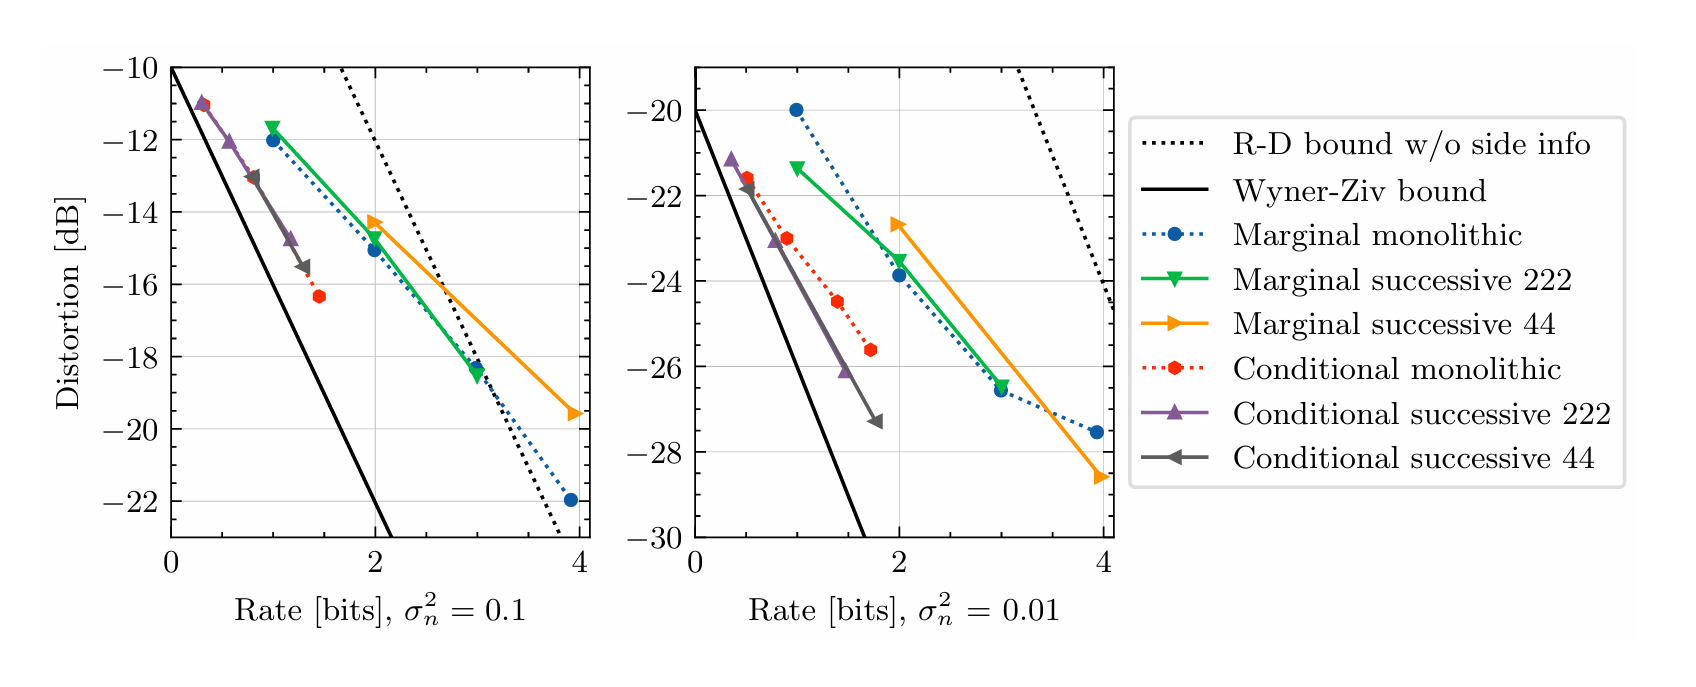
\includegraphics[width=1\textwidth]{Chapters/chapter_1_intro/figures/layered_wz_impovemnts}
    \caption{As seen, the layered WZ quantizer improves the rate-distortion trade-off when using conditional prior, compared to the monolithic WZ quantizer from \cite{OzyilkanRecoverBinning}. The data follows a Gaussian distribution with noise variance of 0.1 or 0.01.}
    \label{fig:layered_wz_improvements}
\end{figure}

\begin{figure}[H]
    \centering
    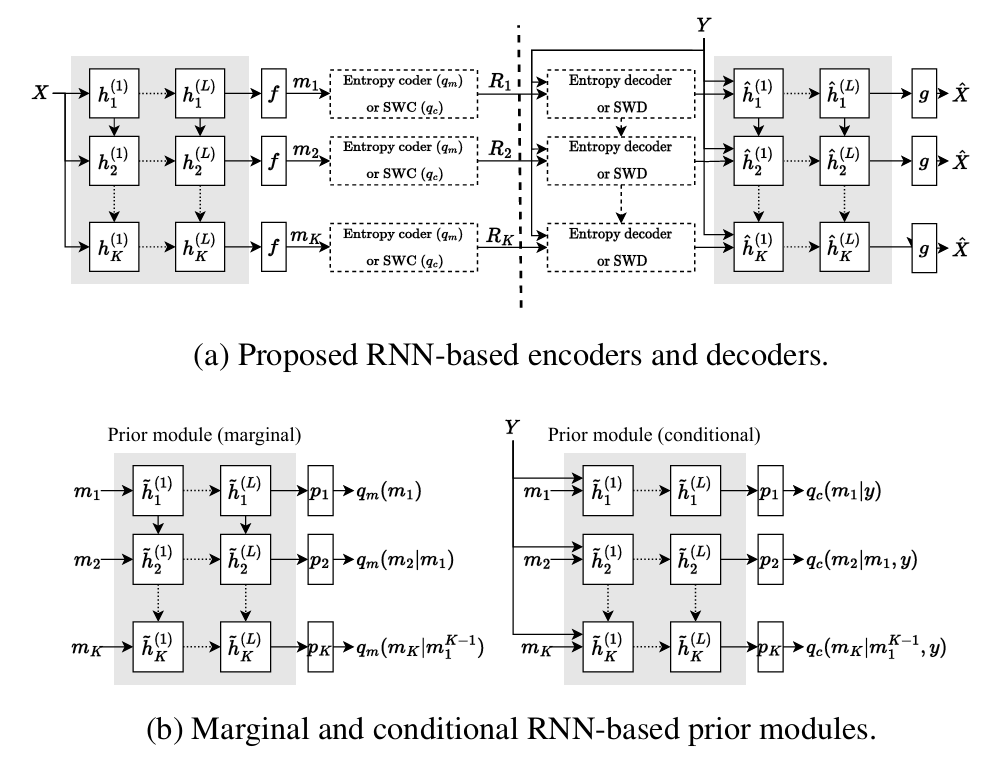
\includegraphics[width=1\textwidth]{Chapters/chapter_1_intro/figures/layered_wz_architecture}
    \caption{The successive refinement architecture of the layered WZ quantizer.}
    \label{fig:layered_wz_architecture}
\end{figure}
